\begin{figure}[htbp]
\centering
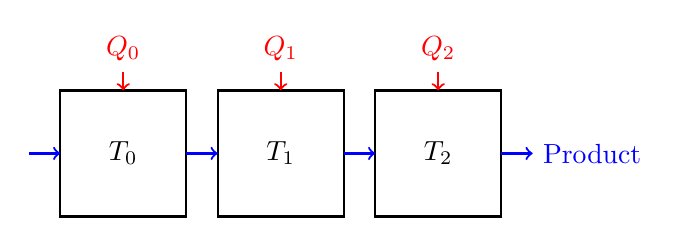
\begin{tikzpicture}[scale=0.8]
    % Zones
    \foreach \i in {0,1,2} {
        \draw[thick] (\i*2.5,0) rectangle (\i*2.5+2,2);
        \node at (\i*2.5+1,1) {$T_\i$};
        \draw[->, thick, red] (\i*2.5+1,2.3) -- (\i*2.5+1,2) node[above, pos=0] {$Q_\i$};
    }

    % Product flow
    \draw[->, thick, blue] (-0.5,1) -- (0,1);
    \draw[->, thick, blue] (2,1) -- (2.5,1);
    \draw[->, thick, blue] (4.5,1) -- (5,1);
    \draw[->, thick, blue] (7,1) -- (7.5,1) node[right] {Product};
\end{tikzpicture}
\caption{Multi-zone temperature control.}
\label{fig:temp_zones}
\end{figure}
